\documentclass{article}


\usepackage{arxiv}

\usepackage[utf8]{inputenc}
\usepackage[dvipsnames]{xcolor}
\usepackage{mathtools, bm}
\usepackage{amssymb, bm}
\usepackage{amsfonts}
\usepackage{fontenc}
\usepackage{amsmath}    
\usepackage{multirow}
\usepackage{mathabx}
\usepackage{fancybox,framed}
\usepackage[T1]{fontenc}
\usepackage{caption}
\usepackage{subcaption}
\usepackage{textcomp}
\usepackage{nicematrix}
\usepackage{xcolor}
\usepackage{bm}
\usepackage{breqn}
\usepackage{listings}
\usepackage{indentfirst}
\usepackage{array}
\usepackage{graphicx}
\usepackage{eso-pic}
\usepackage{float}
% \usepackage{gensymb}
\usepackage{dsfont}
\usepackage{fancybox,framed}
\usepackage{epigraph}
\usepackage{titlesec}
\usepackage{pgf}
\usepackage{tikz}
\usetikzlibrary{arrows.meta}
% \usepackage{biblatex} %Imports biblatex package
\usepackage[backend=biber, defernumbers=true]{biblatex}
\usepackage{wrapfig}
\usepackage{lipsum}
\usepackage{placeins}
\usepackage{appendix}
\usepackage{pgfplots}
\usepackage{algorithm}
\usepackage{algpseudocode}
% hyperref doit être chargé en dernier
\usepackage[colorlinks]{hyperref}



\usepackage[utf8]{inputenc} % allow utf-8 input
\usepackage[T1]{fontenc}    % use 8-bit T1 fonts
\usepackage{hyperref}       % hyperlinks
\usepackage{url}            % simple URL typesetting
\usepackage{booktabs}       % professional-quality tables
\usepackage{amsfonts}       % blackboard math symbols
\usepackage{nicefrac}       % compact symbols for 1/2, etc.
\usepackage{microtype}      % microtypography
\usepackage{lipsum}
\usepackage{graphicx}
\graphicspath{ {./figures/} }

\title{Numerical computation of Hadamard finite part of some hypersingular integrals in 1, 2 and 3 dimensions}

\author{
 Ziyue Qi \\
  School of Coumputing and Information\\
  University of Pittsburgh\\
  Pittsburgh, PA 15213 \\
  \texttt{ziq2@pitt.edu} \\
  %% examples of more authors
   \And
 Zixuan Lu \\
  School of Coumputing and Information\\
  University of Pittsburgh\\
  Pittsburgh, PA 15213 \\
  \texttt{ZIL50@pitt.edu} \\
  \And
 Yuchen Lu \\
  School of Coumputing and Information\\
  University of Pittsburgh\\
  Pittsburgh, PA 15213 \\
  \texttt{yul217@pitt.edu} \\
  %% \AND
  %% Coauthor \\
  %% Affiliation \\
  %% Address \\
  %% \texttt{email} \\
  %% \And
  %% Coauthor \\
  %% Affiliation \\
  %% Address \\
  %% \texttt{email} \\
  %% \And
  %% Coauthor \\
  %% Affiliation \\
  %% Address \\
  %% \texttt{email} \\
}

\begin{document}

\def\Xint#1{\mathchoice
   {\XXint\displaystyle\textstyle{#1}}%
   {\XXint\textstyle\scriptstyle{#1}}%
   {\XXint\scriptstyle\scriptscriptstyle{#1}}%
   {\XXint\scriptscriptstyle\scriptscriptstyle{#1}}%
   \!\int}
\def\XXint#1#2#3{{\setbox0=\hbox{$#1{#2#3}{\int}$}
     \vcenter{\hbox{$#2#3$}}\kern-.5\wd0}}
\def\ddashint{\Xint=}
\def\dashint{\Xint-}

\newtheorem{theorem}{Theorem}[section]
\newtheorem{lemma}{Lemma}[section]
\newtheorem{corollary}{Corollary}[section]
\newtheorem{proposition}{Proposition}[section]

\theoremstyle{definition}
\newtheorem{definition}{Definition}[section]

\theoremstyle{remark}
\newtheorem{remark}{Remark}[section]

\maketitle
\begin{abstract}

\end{abstract}


% keywords can be removed
%\keywords{First keyword \and Second keyword \and More}

\section{Introduction}

\section{Notations}
For every physical quantity, the corresponding reference space quantity is denoted by a hat, so that, for example, if $\mathbf x$ is a point on a $d$-dimensional variety, then $\hat{\mathbf x}$ is the corresponding point in the reference space. If $u$ is a function defined on the variety, then $\hat{u}$ is the corresponding function in the reference space. Furthermore, we denote by $\ddashint$ the Hadamard finite part of an integral.

\textsc{Combinatory notations}: as in the article \cite{constantine_multivariate_1996}, we will use the following notations for multi-indices and combinatory numbers. If $\bm\nu = (\nu_1, \dots, \nu_r) \in \mathbb N_0^r$ and $\bm z = (z_1, \dots, z_r) \in \mathbb R^r$, then

\begin{equation}
  |\bm\nu| = \sum_{i=1}^{r}\nu_i, \qquad \bm\nu! = \prod_{i=1}^{r}\nu_i!, \qquad \bm z^{\bm\nu} = \prod_{i=1}^{r}z_i^{\nu_i}, \qquad \partial^{\bm\nu}_{\bm x} = \frac{\partial^{|\bm\nu|}}{\partial x_1^{\nu_1}\cdots \partial x_r^{\nu_r}}
\end{equation}

as well as the following combinatory sets:

\begin{equation}
  p(n, k) = \left\{(\lambda_1, \dots, \lambda_k):\lambda_i\in\mathbb N_0, \sum_{i=1}^{k} \lambda_i = k, \sum_{i=1}^{k} i\lambda_i = n\right\}
\end{equation}
and its partially vectorized counterparts:
\begin{equation}
\begin{aligned}
p(\bm\nu,r) = \Big\{&(k_1,\dots,k_n;\bm\ell_1,\dots,\bm\ell_n): 
\exists\,1\leq s\leq n:\ \forall\,1\leq i\leq n-s,\\
&k_i=0 \cap \bm\ell_i=\bm 0,\quad 
\forall\,n-s+1\leq i\leq n,\ k_i>0,\\
&\text{et } \bm 0\prec\bm\ell_1\prec\cdots\prec\bm\ell_n
\text{ are such that }\\
&\sum_{i=1}^{n}k_i\bm\ell_i=\bm\nu,\qquad
\sum_{i=1}^{n}k_i=r\Big\}, \qquad n = |\bm\nu|
\end{aligned}
\end{equation}

\begin{equation}
  p(n, \bm\lambda) = \left\{(k_1,\dots,k_n):\bm k_j \leq 0, \sum_{i=1}^{n}\bm k_i=\bm\lambda, \sum_{i=1}^{n}i|\bm k_i|=n\right\}
\end{equation}

Finally, the fully vectorized combinatory set is defined as

\begin{equation}
  p_s(\bm\nu, \bm\lambda) = \left\{((\bm k_1, \dots, \bm k_s); (\ell_1, \dots, \ell_s)): |\bm k_i| > 0, \bm 0 \prec \bm\ell_1\prec\cdots\prec\bm\ell_s, \sum_{i=1}^{s}\bm k_i = \bm\lambda\text{ and }\sum_{i=1}^{s}|\bm k_i|\bm\ell_i = \bm\nu\right\}
\end{equation}

For each of these set, we let the following quantity be defined:

\begin{equation}
  P_{\bm\nu, r} = \sum_{p(\bm\nu, r)}\frac{1}{\prod_{i=1}^{n}k_i!\bm\ell_i!^{k_i}}, \qquad P_{n, \bm\lambda} = \sum_{p(n, \bm\lambda)}\frac{1}{\prod_{i=1}^{n}k_i!i!^{|\bm k_i|}}, \qquad P_{\bm\nu, \bm\lambda}^s = \sum_{p_s(\bm\nu, \bm\lambda)}\frac{1}{\prod_{i=1}^{s}\bm k_i!\bm\ell_i!^{|\bm k_i|}}
\end{equation}

The bold notation will indicate which combinatory set is looked at.

\section{Model presentation}
Let's consider an finite part integral of the form

\begin{equation}
    I = \ddashint_{\hat{\tau}}f(\hat{\mathbf y})\mathrm d\hat{\mathbf y}, \qquad f(\hat{\mathbf y}) \underset{\hat{\mathbf y} \to \hat{\mathbf x}}{\sim} \frac{1}{|| \hat{\mathbf y} - \hat{\mathbf x}||^{d+1}}.
\end{equation}

\section{Injecting Richardson extrapolation into Guiggiani's final formula}
\subsection{Richardson extrapolation - general idea}

For any angle $\theta$, let's consider a finite sequence of $n$ radial points $\rho_i(\theta)$ such that

\begin{equation}
  0 < \rho_1(\theta) < \rho_2(\theta) < \cdots < \rho_n(\theta) < \hat{\rho}(\theta),
\end{equation}

\noindent \textbf{Recall}: we can express the two first terms of the Laurent expansion of the complete polar kernel $F(\rho, \theta) = \rho K(\chi(\hat{\mathbf x}), \chi(\hat{\mathbf y}(\rho, \theta)))J(\hat{\mathbf y}(\rho, \theta))\hat u(\hat{\mathbf y}(\rho, \theta))$ as the following limits

\begin{equation}
  F_{-2}(\theta) = \lim_{\rho \to 0} \rho^2 F(\rho, \theta), \qquad F_{-1}(\theta) = \lim_{\rho \to 0} \rho\left(F(\rho, \theta) - \frac{F_{-2}(\theta)}{\rho^2}\right).
\end{equation}

such that we can write the complete polar kernel as

\begin{equation}
  F(\rho, \theta) = \frac{F_{-2}(\theta)}{\rho^2} + \frac{F_{-1}(\theta)}{\rho} + \underset{\rho\to 1}{\mathcal O}(1)
\end{equation}

Let $c_{1, i}$ and $c_{2, i}$ be the coefficients used in the Richardson extrapolation of order $n$ to compute the previous limits, so that we can write

\begin{equation}
  \boxed{F_{-2}(\theta) \approx \widetilde F_{-2}(\theta) = \sum_{i=1}^{n} c_{2, i} \rho_i^2(\theta) F(\rho_i(\theta), \theta)}, \qquad F_{-1}(\theta) \approx \widetilde F_{-1}(\theta) = \sum_{i=1}^{n} c_{1, i} \rho_i(\theta)\left(F(\rho_i(\theta), \theta) - \frac{\widetilde F_{-2}(\theta)}{\rho_i^2(\theta)}\right).
\end{equation}

By injecting the formula of $\widetilde F_{-2}(\theta)$ into the formula of $\widetilde F_{-1}(\theta)$, so that we can write $\widetilde F_{-1}(\theta)$ only as a linear combination of the complete polar kernel evaluated at the radial points $\rho_i(\theta)$, we obtain

\begin{equation*}
  \widetilde F_{-1}(\theta) = \sum_{i=1}^{n} c_{1, i} \rho_i(\theta) F(\rho_i(\theta), \theta) - \sum_{i=1}^{n} c_{1, i} \frac{1}{\rho_i(\theta)}\sum_{j=1}^{n} c_{2, j} \rho_j^2(\theta) F(\rho_j(\theta), \theta).
\end{equation*}

By letting $P_n(\theta) = \sum_{k=1}^{n}\frac{1}{\rho_k(\theta)}$, we can write the previous formula as

\begin{equation}
  \boxed{\widetilde F_{-1}(\theta) = \sum_{i=1}^{n} F(\rho_i(\theta), \theta)\rho_i(\theta)\Big(c_{1, i} - c_{2, i}P_n(\theta)\rho_i(\theta)\Big)}
\end{equation}

\subsection{Lagrange basis method}

For this section and the following, we will no longer use $\theta$ in the notation, it will be implicit. Let's denote the regular function $G(\rho) = \rho^2 F(\rho)$, so that $G(0) = F_{-2}$ and $G'(0) = F_{-1}$. Let $\ell_i(\rho)$ be the Lagrange basis of degree $n-1$ associated to the radial points $\rho_i$, defined as

\begin{equation}
  \ell_i(\rho) = \prod_{j\neq i}\frac{\rho - \rho_j}{\rho_i - \rho_j}, \qquad i = 1, \dots, n.
\end{equation}

The lagrange interpolant of $G$ and its derivative are given by

\begin{equation}
  \Pi_{n-1}G(\rho) = \sum_{i=1}^{n} G(\rho_i)\ell_i(\rho), \qquad (\Pi_{n-1}G)'(\rho) = \sum_{i=1}^{n} G(\rho_i)\ell_i'(\rho).
\end{equation}

So that the numerical Laurent's coefficients, denoted $\widetilde F_{-2}$ and $\widetilde F_{-1}$, are simply the evaluation of the interpolant and its derivative at the origin $\rho = 0$:

\begin{equation}
  \widetilde F_{-2} = \Pi_{n-1}G(0) = \sum_{i=1}^{n} G(\rho_i)\ell_i(0), \qquad \widetilde F_{-1} = (\Pi_{n-1}G)'(0) = \sum_{i=1}^{n} G(\rho_i)\ell_i'(0).
\end{equation}

with $\displaystyle{\ell_i(0) = \prod_{j\neq i}\frac{\rho_j}{\rho_j - \rho_i}}$ and $\displaystyle{\ell_i'(0) = \ell_i(0)\left(\frac{1}{\rho_i} - P_n\right)}$, so that we can finally write the Laurent's coefficients as

\begin{equation}
  \widetilde F_{-2} = \sum_{i=1}^{n} \ell_i(0)\rho_i^2 F(\rho_i), \qquad \widetilde F_{-1} = \sum_{i=1}^{n} \ell_i(0)\rho_i\left(1 - P_n\rho_i\right)F(\rho_i).
\end{equation}

This is a particular case of the Richardson extrapolation, with the two families of coefficients $c_{1, i}$ and $c_{2, i}$ collapsing into a single family of coefficients $\ell_i(0)$:

$$c_{1, i} = c_{2, i} = \ell_i(0) = c_i = \prod_{j\neq i}\frac{\rho_j}{\rho_j - \rho_i}.$$

Finally, the numerical Laurent's coefficients can be written as

\begin{equation}
  \widetilde F_{-2}(\theta) = \sum_{i=1}^{n}A_i(\theta)F(\rho_i(\theta), \theta), \qquad \widetilde F_{-1}(\theta) = \sum_{i=1}^{n}B_i(\theta)F(\rho_i(\theta), \theta).
\end{equation}

With $A_i(\theta) = c_i(\theta)\rho_i^2(\theta)$ and $B_i(\theta) = c_i(\theta)\rho_i(\theta)\left(1 - P_n(\theta)\rho_i(\theta)\right)$.

Each of these formula simply consist in the numerical evaluation of the polar kernel at the radial points $\rho_i(\theta)$, multiplied by some weights.

\subsubsection{Properties of $A_i(\theta)$ and $B_i(\theta)$}

\begin{equation}
  \sum_{i=1}^{n} A_i = 
  \begin{cases}
    \rho_1, & n = 1 \\
    -\rho_1\rho_2, & n = 2 \\
    0, & n \geq 3
  \end{cases}, \qquad
  \sum_{i=1}^{n} B_i = 
  \begin{cases}
    0, & n = 1 \\
    \rho_1 + \rho_2, & n = 2 \\
    0, & n \geq 3
  \end{cases}
\end{equation}

These three cases illustrates the following definition :

\begin{equation}
  \sum_{i=1}^{n} A_i = (\Pi_{n-1}[\rho^2])(0), \qquad \sum_{i=1}^{n} B_i = (\Pi_{n-1}[\rho^2])'(0)
\end{equation}

\subsection{Final quadrature rule}

Let's then denote $I(\theta)$ the integral of the complete polar kernel over the radial direction, defined as:

\begin{equation}
  I(\theta) = \int_{0}^{\hat{\rho}(\theta)} \left\{F(\rho, \theta) - \frac{F_{-1}(\theta)}{\rho} - \frac{F_{-2}(\theta)}{\rho^2}\right\}\mathrm d\rho + F_{-1}(\theta)\ln\left|\frac{\hat\rho(\theta)}{\beta(\theta)}\right| - F_{-2}(\theta)\left\{\frac{\gamma(\theta)}{\beta^2(\theta)}+\frac{1}{\hat\rho(\theta)}\right\}
\end{equation}

A final quadrature rule for it is the following:

\begin{equation}
  I(\theta) \approx \widetilde I(\theta) = \sum_{i=1}^{n} \widetilde w_i(\theta) F(\rho_i(\theta), \theta)
\end{equation}

With the new weights $\widetilde w_i(\theta)$ defined as

\begin{align*}
  \widetilde{w}_i(\theta) & = w_i(\theta) - A_i(\theta)\left\{W_{-2,n}(\theta) + \frac{\gamma(\theta)}{\beta^2(\theta)} + \frac{1}{\hat\rho(\theta)}\right\} + B_i(\theta)\left\{\ln\left|\frac{\hat\rho(\theta)}{\beta(\theta)}\right| - W_{-1,n}(\theta)\right\}
\end{align*}

and the auxiliary constants : 

\begin{itemize}
  \item $w_i(\theta) = \frac{\hat\rho(\theta)}{2}w_i^{\text{Ref}}$ are the weights of the reference quadrature over the segment $[-1, 1]$.
  \item $W_{-1,n}(\theta) = \sum_{i=1}^{n} \frac{w_i(\theta)}{\rho_i(\theta)} = \sum_{i=1}^{n} \frac{w_i^{\text{Ref}}}{1+x_i^{\text{Ref}}}$.
  \item $W_{-2,n}(\theta) = \sum_{i=1}^{n} \frac{w_i(\theta)}{\rho_i^2(\theta)} = \frac{2}{\hat\rho(\theta)}\sum_{i=1}^{n} \frac{w_i^{\text{Ref}}}{\left(1+x_i^{\text{Ref}}\right)^2}$.
\end{itemize}

\begin{remark} 
  In the case of Gauss-Legendre quadrature, the constants $W_{-1,n}$ and $W_{-2,n}$ can be computed analytically as:  

  \begin{equation}
    W_{-1,n} = 2H_n, \qquad W_{-2,n}(\theta) = \frac{2}{\hat\rho(\theta)}n(n+1), \qquad P_n(\theta) = \frac{n(n+1)}{\hat\rho(\theta)}
  \end{equation}

  With $H_n = \sum_{i=1}^{n} \frac{1}{i}$ the $n$-th harmonic number. These last two formulas are, for the moment, a conjecture. (Elaborate to prove it?)

\end{remark}

\begin{remark} Properties of the new weights $\widetilde w_i(\theta)$
    
  \begin{equation}
    \text{For } n \geq 3, \quad
    \sum_{i=1}^{n} \widetilde w_i(\theta) = \hat\rho(\theta)
  \end{equation}

  This is easy to understand: either look at the definition of $\widetilde w_i(\theta)$ and use the properties of $A_i(\theta)$ and $B_i(\theta)$, or integrate the constant function $F(\rho, \theta) = 1$ between $0$ and $\hat\rho(\theta)$, which is equivalent. In a more general way, if the integrand $F$ is not singular (i.e. $F \sim \mathcal O(1)$), then the quadrature rule is the standard quadrature as if reference quadrature was used to integrate the function $F$ between $0$ and $\hat\rho(\theta)$. If the integrand is singular as $1/\rho$, the customed quadrature just performs a Cauchy principal value. The true ingredients are the values of the Laurent coefficients $F_{-1}$ and $F_{-2}$, which are computed numerically; they can be zero (up to the algorithm precision) or not, depending on the considered singularity.
  
\end{remark}

\subsection{Convergence and error study}

\subsubsection{General idea}
\label{sec:bernstein-R}

To begin our reasoning, assume that we have computed the Laurent's coefficients up to a relative error $\epsilon_{-k}$, $k\in\{1, 2\}$:

\begin{equation}
  \widetilde F_{-k} = F_{-k}(1+\epsilon_{-k}), \qquad k\in\{1, 2\}
\end{equation}

Now let's denote

\begin{align}
  R(\rho, \theta) & = F(\rho, \theta) - \frac{F_{-1}(\theta)}{\rho} - \frac{F_{-2}(\theta)}{\rho^2} \\
\widetilde R(\rho, \theta) & = F(\rho, \theta) - \frac{\widetilde F_{-1}(\theta)}{\rho} - \frac{\widetilde F_{-2}(\theta)}{\rho^2} \\
\end{align}

\begin{equation}
  I = \int_{0}^{2\pi}\int_{0}^{\hat\rho(\theta)}R(\rho, \theta)\mathrm d\rho\mathrm d\theta, \qquad \widetilde I = \int_{0}^{2\pi}\int_{0}^{\hat\rho(\theta)}\widetilde R(\rho, \theta)\mathrm d\rho\mathrm d\theta
\end{equation}

On one hand, after the theory of the Bernstein's ellipses, if we assume that $R$ and $\widetilde R$ are analytic, we can make a error majoration regarding the Gauss-Legendre quadrature of $I$ and $\widetilde I$:

\begin{align}
  \left|I - Q_n[R]\right| & \leq \frac{64}{15}\frac{M}{(1 - \rho_B^{-2})\rho_B^{2n}} \\
  \left|\widetilde I - Q_n[\widetilde R]\right| & \leq \frac{64}{15}\frac{\widetilde M}{(1 - \widetilde \rho_B^{-2})\widetilde \rho_B^{2n}}
\end{align}

On the other hand, we can substract $\widetilde I$ to $I$ to get:

\begin{equation}
  |I - \widetilde I| \leq C(\hat x) \sum_{k=1}^2\frac{\epsilon_{-k}}{\rho_{\min}^k}||F_{-k}||_{\infty}
\end{equation}

where $\displaystyle{C(\hat x) = \int_{0}^{2\pi}\hat\rho(\theta)\mathrm d\theta}$.

Thus, 

\begin{align}
  |I - Q_n[\widetilde R]| & = |I - \widetilde I + \widetilde I - Q_n[\widetilde R]| & \leq |I - \widetilde I| + |\widetilde I - Q_n[\widetilde R]| & \leq C(\hat x) \sum_{k=1}^2\frac{\epsilon_{-k}}{\rho_{\min}^k}||F_{-k}||_{\infty} + \frac{64}{15}\frac{\widetilde M}{(1 - \widetilde \rho_B^{-2})\widetilde \rho_B^{2n}}
\end{align}

\subsubsection{Richardson extrapolation}

\begin{lemma}\label{lemma:convergence_Richardson}
  
  We can show that the following majorations hold for any sequence $\rho_i(\theta)$ of $n$ radial points:

  \begin{equation}
    |\widetilde F_{-2} - F_{-2}| \leq \frac{||\partial^n_\rho G||_{\infty}}{n!}\prod_{i=1}^{n}\rho_i, \qquad |\widetilde F_{-1} - F_{-1}| \leq \left\{\frac{\left\|\partial_\rho^{n+1}G\right\|_{\infty}}{(n+1)!}+P_n\frac{\left\|\partial_\rho^{n}G\right\|_{\infty}}{n!}\right\}\prod_{i=1}^{n}\rho_i
  \end{equation}

\end{lemma}

  Which shows that the speed of convergence is conditionned by the product of the radial points $\prod_{i=1}^{n}\rho_i(\theta)$. In the case of a geometric sequence $\rho_i(\theta) = \hat\rho(\theta)q^{i-1}$, we have $\prod_{i=1}^{n}\rho_i(\theta) = \hat\rho^n(\theta)q^{\frac{n(n-1)}{2}}$, which is a very fast convergence. In the case of a sequence of Gauss-Legendre quadrature points, we have $\prod_{i=1}^{n}\rho_i(\theta) = \hat\rho^n(\theta)\frac{(n!)^2}{(2n)!}$, which is a slower convergence\footnote{We need to qualify this statement} (see Figures \ref{fig:convergence_comparison_F2_realist}, \ref{fig:convergence_comparison_F1_realist}, \ref{fig:convergence_comparison_F2_ideal} and \ref{fig:convergence_comparison_F1_ideal}).

\begin{figure}
  \centering
  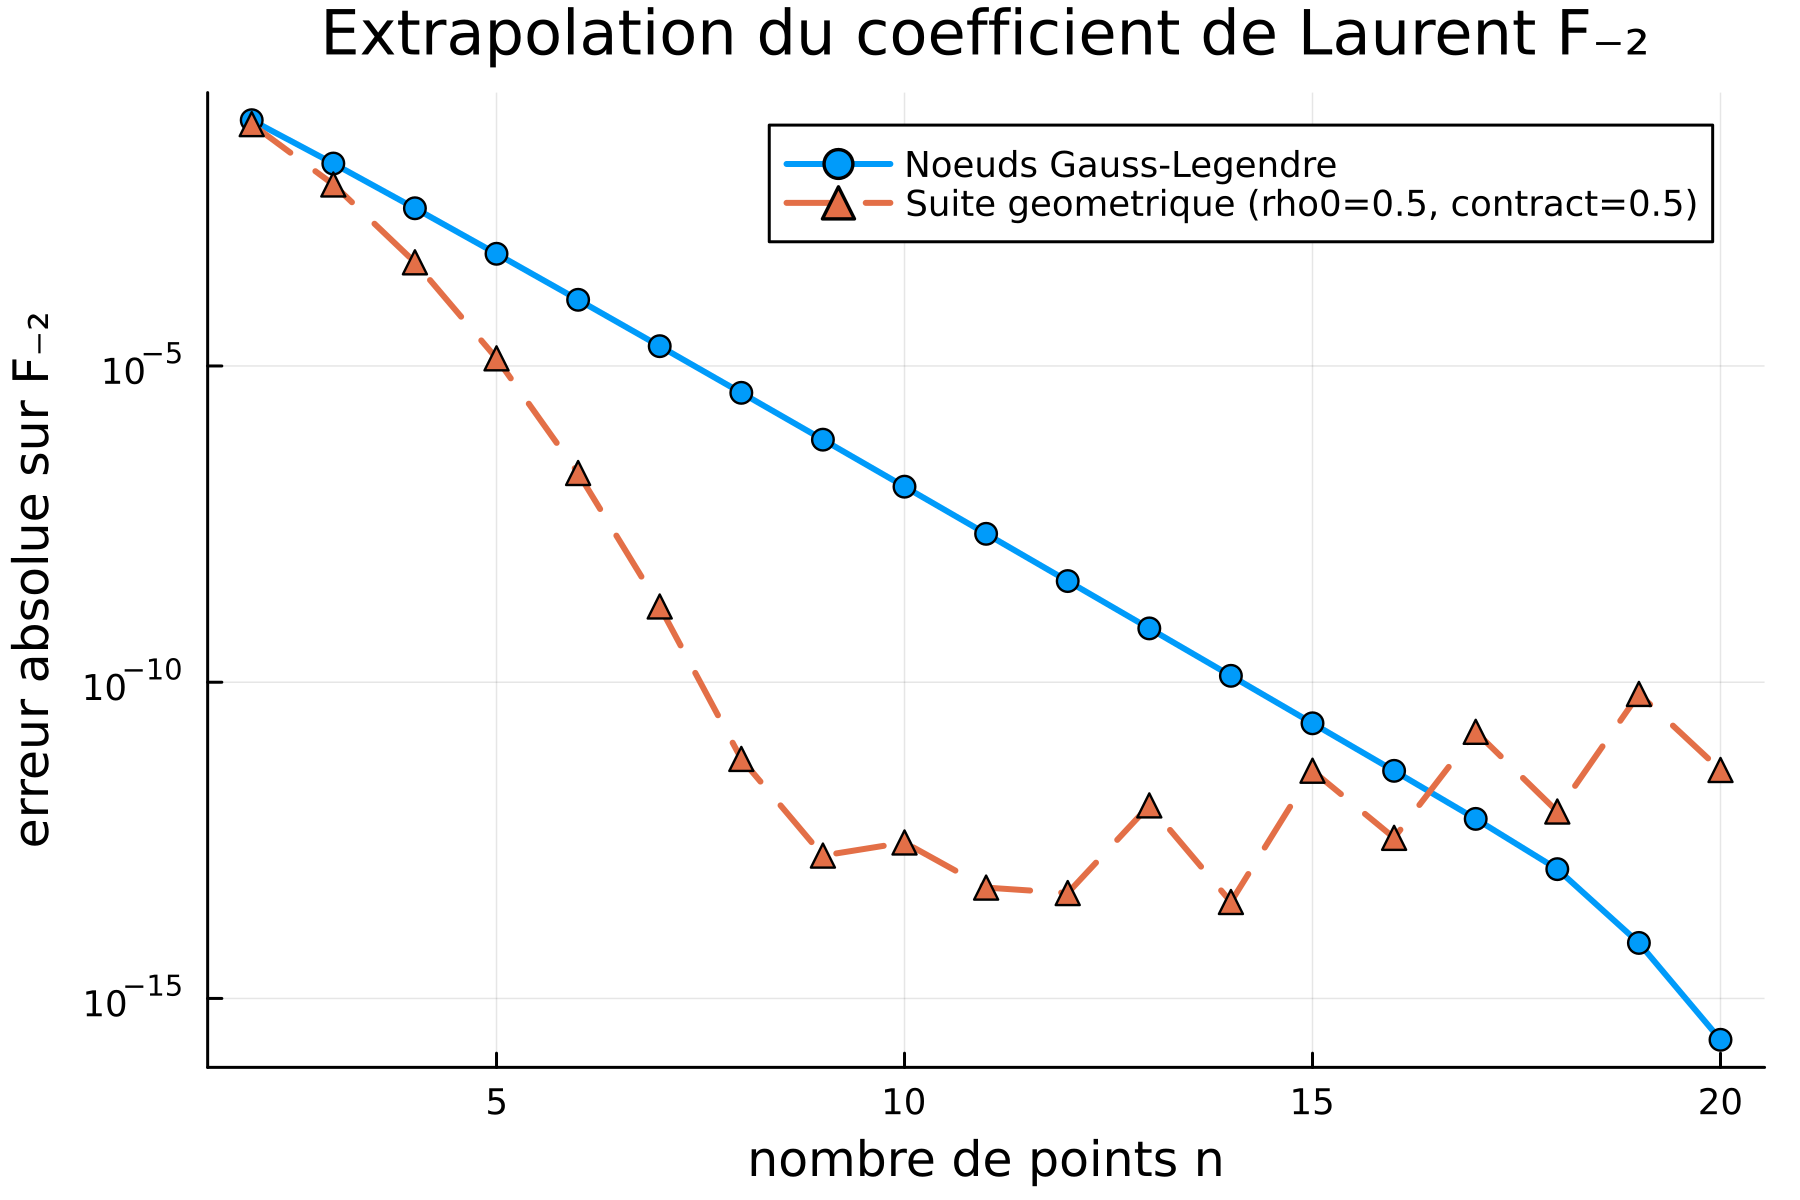
\includegraphics[width=0.8\textwidth]{figures/gl_vs_geometric_extrapolation_F2_realist.png}
  \caption{Convergence comparison between geometric and Gauss-Legendre sequences for the function $\rho\to \rho^2\times 1/(\rho^2(1+\rho))$ (realistic case)}
  \label{fig:convergence_comparison_F2_realist}
\end{figure}

\begin{figure}
  \centering
  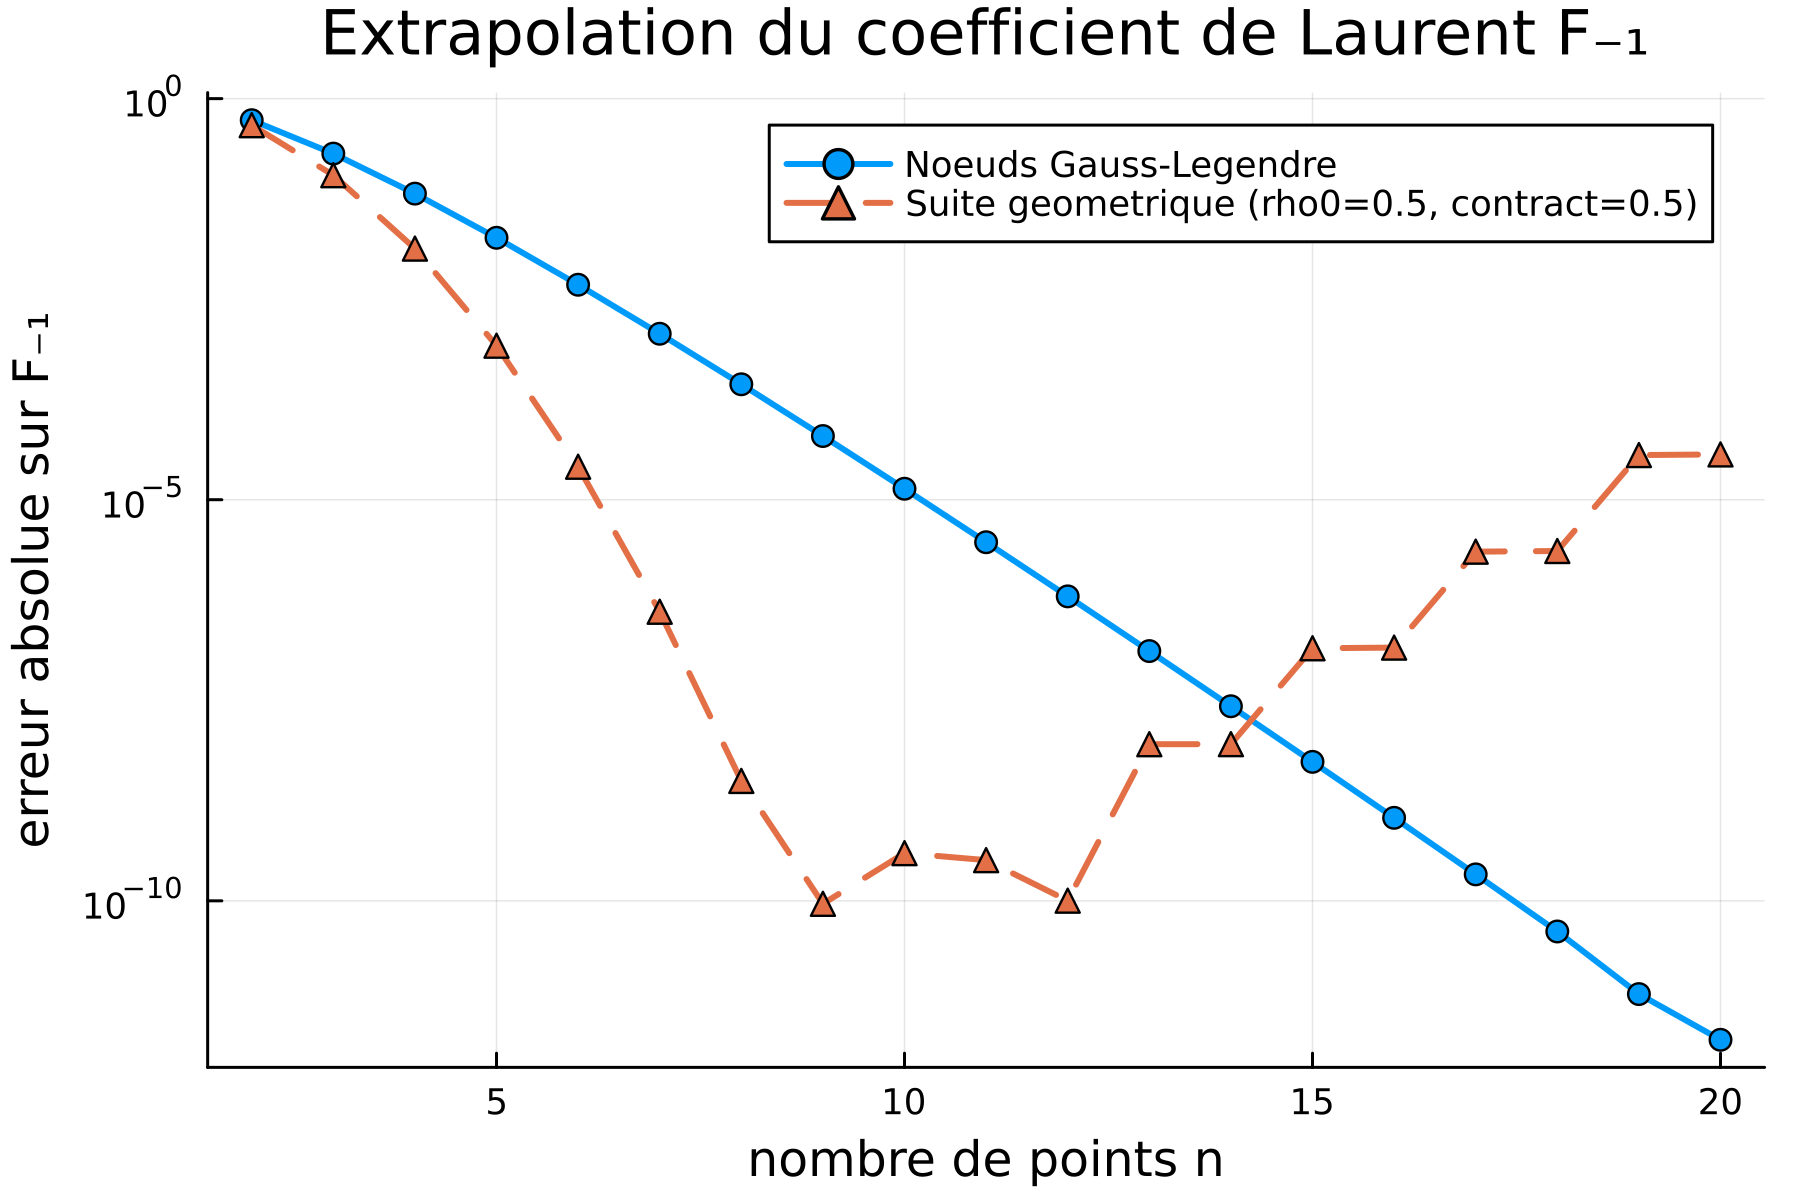
\includegraphics[width=0.8\textwidth]{figures/gl_vs_geometric_extrapolationF1_realist.png}
  \caption{Convergence comparison between geometric and Gauss-Legendre sequences for the function $\rho\to \rho^2\times 1/(\rho^2(1+\rho))$ (realistic case)}
  \label{fig:convergence_comparison_F1_realist}
\end{figure}

\begin{figure}
  \centering
  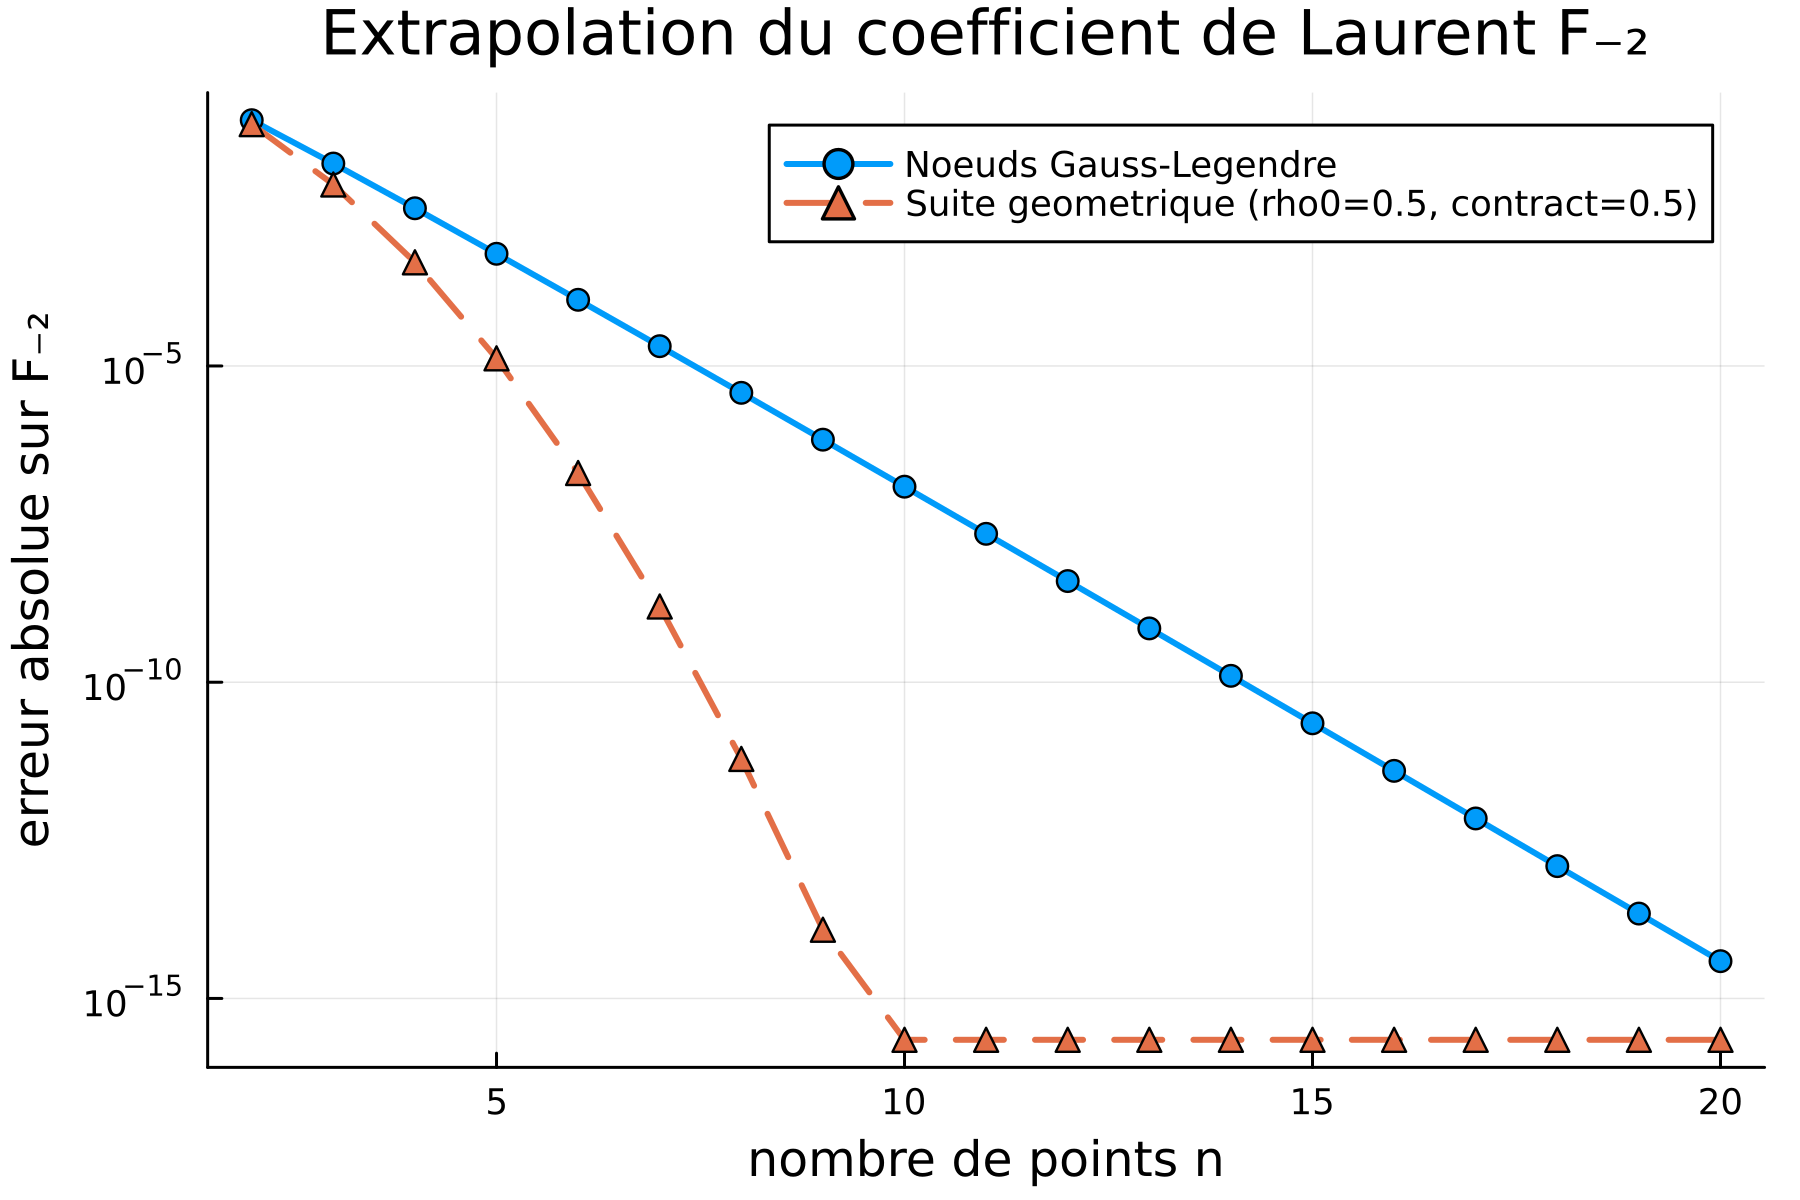
\includegraphics[width=0.8\textwidth]{figures/gl_vs_geometric_extrapolation_F2_ideal.png}
  \caption{Convergence comparison between geometric and Gauss-Legendre sequences for the function $\rho\to 1/(1+\rho)$ (ideal case)}
  \label{fig:convergence_comparison_F2_ideal}
\end{figure}

\begin{figure}
  \centering
  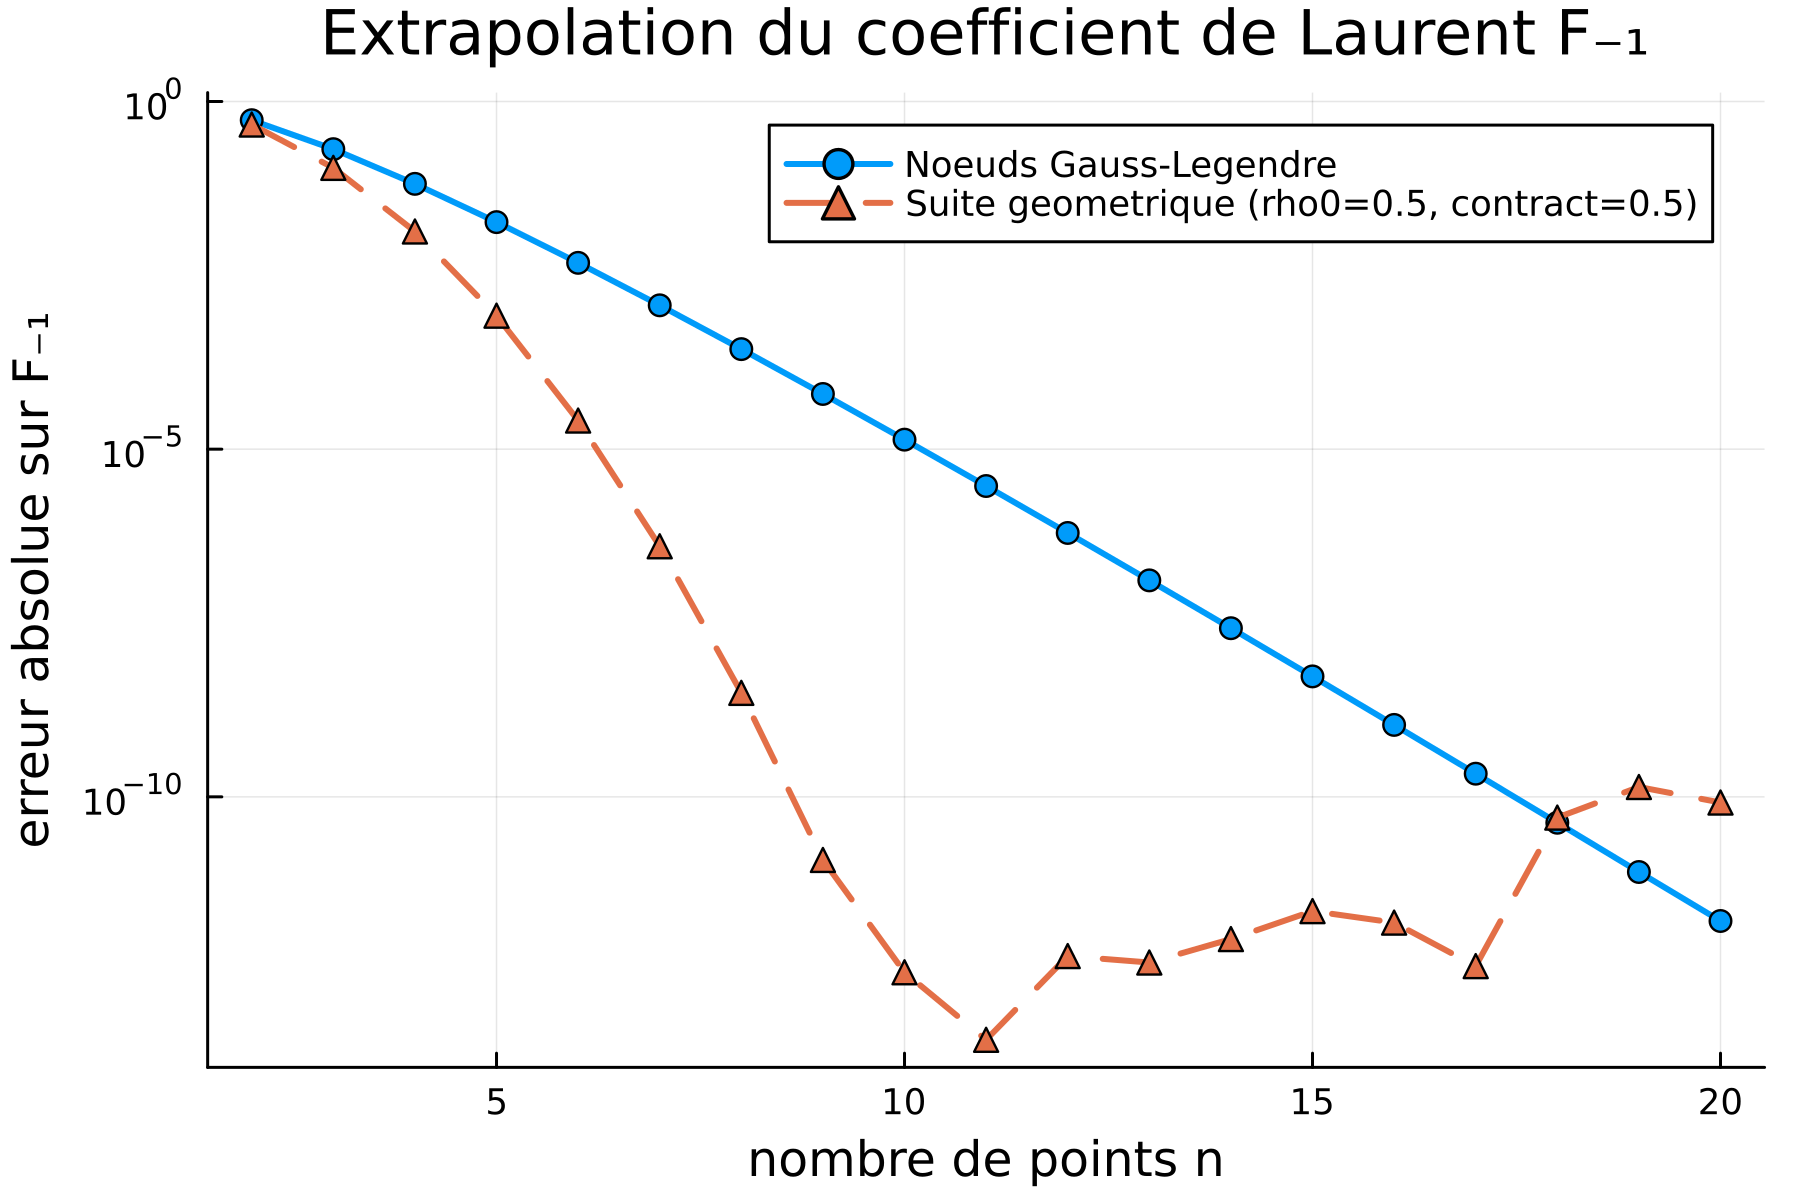
\includegraphics[width=0.8\textwidth]{figures/gl_vs_geometric_extrapolationF1_ideal.png}
  \caption{Convergence comparison between geometric and Gauss-Legendre sequences for the function $\rho\to 1/(1+\rho)$ (ideal case)}
  \label{fig:convergence_comparison_F1_ideal}
\end{figure}

That's why geometric sequences can be preferred over Gauss-Legendre quadrature points for pure Richardson extrapolation.

\begin{proof}[Proof of lemma \ref{lemma:convergence_Richardson}] Let $e(\rho) = G(\rho) - \Pi_{n-1}G(\rho)$ be the interpolation error of $G$ by its Lagrange interpolant $\Pi_{n-1}G$. We have the following formula for the interpolation error, which is quite general on polynomial interpolation:

\begin{equation}
  e(\rho) = G[\rho_1, \cdots, \rho_n, \rho]\prod_{i=1}^{n}(\rho - \rho_i)
\end{equation}

Where $G[\rho_1, \cdots, \rho_n, \rho]$ is the divided difference of order $n$ of $G$ at the points $\rho_1, \cdots, \rho_n, \rho$. By using the mean value theorem for divided differences, we can write

\begin{equation}
  G[\rho_1, \cdots, \rho_n, \rho] = \frac{G^{(n)}(\xi)}{n!}
\end{equation}

For some $\xi \in [0, \hat\rho]$. Thus, we can write 

\begin{equation}
  \left|\widetilde F_{-2} - F_{-2}\right| = \left|e(0)\right| \leq \frac{||\partial^n_\rho G||_{\infty}}{n!}\prod_{i=1}^{n}\rho_i
\end{equation}

Then, taking the derivative of the interpolation error, we have

\begin{align*}
  e'(\rho) & = \partial_\rho\left\{G[\rho_1, \cdots, \rho_n, \rho]\prod_{i=1}^{n}(\rho - \rho_i)\right\} \\
  & = \partial_\rho\left\{G[\rho_1, \cdots, \rho_n, \rho]\right\}\prod_{i=1}^{n}(\rho - \rho_i) + G[\rho_1, \cdots, \rho_n, \rho]\partial_\rho\left\{\prod_{i=1}^{n}(\rho - \rho_i)\right\} \\
  & = G[\rho_1, \cdots, \rho_n, \rho, \rho]\prod_{i=1}^{n}(\rho - \rho_i) + G[\rho_1, \cdots, \rho_n, \rho]P_n\prod_{i=1}^{n}(\rho - \rho_i) \\
  \left|\widetilde F_{-1} - F_{-1}\right| = \left|e'(0)\right| & \leq \left\{\frac{\left\|\partial_\rho^{n+1}G\right\|_{\infty}}{(n+1)!}+P_n\frac{\left\|\partial_\rho^{n}G\right\|_{\infty}}{n!}\right\}\prod_{i=1}^{n}\rho_i
\end{align*}

using again the mean value theorem for $G[\rho_1, \cdots, \rho_n, \rho]$ and $G[\rho_1, \cdots, \rho_n, \rho, \rho]$.

\end{proof}

\subsubsection{Gauss-Legendre quadrature}

To delve deeper into these general ideas, let's consider :

\begin{align}
  \widetilde I_{\epsilon,h,n}(\theta) & = Q_n[\widetilde R_{\epsilon, h}](\theta) = \sum_{i=1}^{n} w_i(\theta) \left\{F_h(\rho_i(\theta), \theta) - \frac{\widetilde F_{-1, \epsilon, h}(\theta)}{\rho_i(\theta)} - \frac{\widetilde F_{-2, \epsilon, h}(\theta)}{\rho_i^2(\theta)}\right\} \\
& = \sum_{i=1}^{n}\left\{F_h(\rho_i(\theta), \theta) - \frac{F_{-1, h}(\theta)}{\rho_i(\theta)} - \frac{F_{-2, h}(\theta)}{\rho_i^2(\theta)}\right\}w_i(\theta) - \sum_{k=1}^{2}F_{-k, h}(\theta)\epsilon_{-k}\sum_{i=1}^{n}\frac{w_i(\theta)}{\rho_i^k(\theta)} \\
& = Q_n[R_h](\theta) - \sum_{k=1}^{2}F_{-k, h}(\theta)\epsilon_{-k}W_{-k,n}(\theta)
\end{align}

Where $h$ is the mesh size. Thanks to standard results on the Gauss-Legendre quadrature for any function in $\mathcal C^{2n}([0, \hat\rho(\theta)])$, we have the following error majoration (deleting the $\theta$ dependency for clarity):

\begin{equation}
  Q_n[R_h] = \int_{0}^{\hat\rho}R_h(\rho)\mathrm d\rho + \frac{2^{2n+1}(n!)^4}{(2n+1)[(2n)!]^3}R_h^{(2n)}(\rho_0)
\end{equation}

for some $\rho_0 \in [0, \hat\rho]$. Our next goal is to show that the error term $R_h^{(2n)}(\rho_0)$ converges with the mesh size $h$ and the number of quadrature points $n$. By using $G_h(\rho) = \rho^2 F_h(\rho) = \mathcal O_{\rho\to 0}(1)$, we can straightforwardly express $R_h$ in terms of $G$, and bound its derivatives, assuming, as Guiggiani, that $F_h$ is analytic in a neighborhood of the origin:

\begin{align}
  R_h(\rho) & = \sum_{k=0}^{+\infty}F_k\rho^k, \qquad \Longrightarrow \qquad R_h^{(2n)}(\rho) = \sum_{k=2n}^{+\infty}F_k\frac{k!}{(k-2n)!}\rho^{k-2n} \\
\end{align}

with $\displaystyle{F_k = \frac{G_h^{(k+2)}(0)}{(k+2)!} \leq \frac{1}{(k+2)!}||G_h^{(k+2)}||_{\infty, [0, \hat\rho]}}$ and $\rho^{k-2n} \leq \hat\rho^{k-2n}$, so that we can write

\begin{equation}
  |R_h^{(2n)}(\rho)| \leq \sum_{k=2n}^{+\infty}k!\frac{||G_h^{(k+2)}||_{\infty, [0, \hat\rho]}}{(k+2)!(k-2n)!}\hat\rho^{k-2n}
\end{equation}

\subsubsection{Derivation of the regularized kernel $G$ with respect to $\rho$}

In this section, we will explicitely estimate $\partial^mG$ using complete chain rules derivatives in terms of the mesh size $h$, which corresponds to the size of the physical element $\tau$ in the physical space ; taking, for instance, the radius of the circumscribed circle of an arbitrary element $\tau$ of the mesh.

\begin{definition} Let us first defined the following functions:
  
$$\begin{array}{ccccc}
\phi_h & : & \hat\tau\subset\mathbb R^{d-1} & \to & \mathbb R \\
 & & \hat x & \mapsto & \det M_h(\hat x) \\
\end{array}, \qquad \begin{array}{ccccc}
\psi_{\hat x} & : & \mathbb R\times [0, 2\pi[ & \to & \mathbb R^{d-1} \\
 & & (\rho, \theta) & \mapsto &\hat x + \rho \mathbf u(\theta) \\
 \end{array}\\$$

$$\begin{array}{ccccc}
\chi_h & : & \hat\tau\subset\mathbb R^{d-1} & \to & \tau\subset\mathbb R^d\\
 & & \hat x & \mapsto & x \\
\end{array}$$

where $\chi$ is the mapping from the reference space to the physical element, $\psi_{\hat x}$ is the mapping from polar coordinates to the reference space, and $M_h$ is the metric tensor of the mapping $\chi_h$, defined as:

\begin{equation}
  M_h(\hat x) = D\chi_h(\hat x)^TD\chi_h(\hat x), \qquad (M_h)_{ab} = \sum_{k=1}^{d}\frac{\partial\chi_{h,k}}{\partial \hat x_a}\frac{\partial\chi_{h,k}}{\partial \hat x_b}, \quad (a, b)\in \{1, \dots, d-1\}^2 = \{1, 2\}^2
\end{equation}

Finally, the vector $\mathbf u(\theta)$ is the unit trigonometric vector defined as $\mathbf u(\theta) = (\cos\theta, \sin\theta)$ for our case $d = 3$. 
\end{definition}

\begin{lemma}\label{lemma:FaadiBruno-polar}
  
Using the Faà di Bruno formula for functions of the form $h(x) = f[g_1(x), \dots, g_m(x)]$ (see \cite{constantine_multivariate_1996}), one can write, for any function $f : \mathbb R^{2} \to \mathbb R$,

\begin{equation}\label{eq:FaadiBruno-polar}
  \partial^k_{\rho} (f\circ\psi_{\hat x})(\rho, \theta) = \sum_{i=0}^{k}\binom{k}{i}\cos^i(\theta)\sin^{k-i}(\theta)\frac{\partial^k f}{\partial \hat x_1^i\partial \hat x_2^{k-i}}(\psi_{\hat x}(\rho, \theta))
\end{equation}
\end{lemma}

We can then expand $G$ as

\begin{equation}
  G(\rho, \theta) = H_h(\rho, \theta)J_h\circ\psi_{\hat x}(\rho, \theta)
\end{equation}

where

\begin{equation}\label{eq:Hh-def}
  H_h(\rho, \theta) = \rho^3K\Big(x = \chi_h(\hat x), y = \chi_h\circ\psi_{\hat x}(\rho, \theta)\Big)\hat u\circ\psi_{\hat x}(\rho, \theta), \quad J_h(\hat x) = \sqrt{\phi_h(\hat x)} = \sqrt{\det M_h(\hat x)}
\end{equation}


\begin{lemma}\label{lemma:factorization-radius}
  We have the following useful factorization:

\begin{equation}
  \bm r = \rho\bm A_{\hat x}(\rho, \theta), \quad \bm A_{\hat x}(\rho, \theta) = \sum_{m\geq 1}\frac{\rho^{m-1}}{m!}D^m\chi_h(\hat x):_m\left(\bm u(\theta)^{m\otimes}\right)
\end{equation}
\end{lemma}

\textbf{Homogeneous kernels}. When the kernel is homogeneous, i.e 

$$\exists \hat K, K(x, y) = \frac{1}{r^s}\hat K(\mathbf{\hat r}, n_x, n_y), \quad\forall n_x, n_y \in \mathbb S^{d}, z\to \hat K(z, n_x, n_y) \text{ is of class } \mathcal C^{\infty}(\mathbb R^d)$$
\begin{align}\label{ineq:reg-pol-kernel}
  \text{i.e } \forall \alpha\in\mathbb N^d, \quad \exists C_K(|\alpha|) > 0, \quad \left|\frac{\partial^{|\alpha|}\hat K}{\partial z^{\alpha}}(z, n_x, n_y)\right| \leq C_K(|\alpha|), \quad \forall z\in\mathbb R^d
\end{align}

Then we have 

\begin{align}\label{eq:reg-pol-kernel}
  \rho^s K(\chi_h(\hat x), \chi_h\circ\psi_{\hat x}(\rho, \theta))
  & = \left(\frac{\rho}{r}\right)^s
  \hat K\!\left(\hat{\mathbf A}_{\hat x}(\rho, \theta),
  n\circ\chi_h(\hat x),
  n\circ\chi_h\circ\psi_{\hat x}(\rho,\theta)\right) \\
  & = \frac{1}{\left\|\bm A_{\hat x}(\rho, \theta)\right\|^s}
  \hat K\!\left(\hat{\mathbf A}_{\hat x}(\rho, \theta),
  n\circ\chi_h(\hat x),
  n\circ\chi_h\circ\psi_{\hat x}(\rho,\theta)\right) \\
  & = A_{\hat x}(\rho, \theta)^{-s}
  \hat K\!\left(\hat{\mathbf A}_{\hat x}(\rho, \theta),
  n\circ\chi_h(\hat x),
  n\circ\chi_h\circ\psi_{\hat x}(\rho,\theta)\right)
\end{align}

Where $s$ is the order of singularity of the function $\rho\to K(\chi_h(\hat x), \chi_h\circ\psi_{\hat x}(\rho, \theta))$ at the origin, such that $K(\chi_h(\hat x), \chi_h\circ\psi_{\hat x}(\rho, \theta)) = \mathcal O_{\rho\to 0}(\rho^{-s})$. The idea was originally used for hypersingular 3D kernels, where $s = 3$ (see Guiggiani, 1992), but we write the computations with general order $s$ because the idea remains the same.

We will denote $\hat K\!\left(\hat{\mathbf A}_{\hat x}(\rho, \theta),
  n\circ\chi_h(\hat x),
  n\circ\chi_h\circ\psi_{\hat x}(\rho,\theta)\right)$ as $\hat K_{\hat x}(\rho, \theta)$ for clarity, keeping in mind that this is the kernel evaluated in polar coordinates in parameter space centered at point $\hat x$.

As the kernel $K$ is regularized by the term $\rho^3$ in $H_h$, we can ensure that $H_h = \mathcal O_{\rho\to 0} (1)$. Applying the Leipniz formula, we have

\begin{equation}
  \partial^m_{\rho}G(\rho, \theta) = \sum_{k=0}^{m}\binom{m}{k} \partial^k_{\rho} H_h(\rho, \theta) \partial^{m-k}_{\rho}(J_h\circ\psi_{\hat x})(\rho, \theta)
\end{equation}

With:

\begin{align*}
  \partial_{\rho}^{k}H_h(\rho, \theta) & = \sum_{i=0}^{k}\binom{k}{i}\partial^{i}_{\rho}\left(A_{\hat x}(\rho, \theta)^{-s}\hat K_{\hat x}(\rho, \theta)\right)\partial^{k-i}_\rho(\hat u\circ\psi_{\hat x})(\rho, \theta) \\
  \partial_{\rho}^{m-k}(J_h\circ\psi_{\hat x})(\rho, \theta) & \leq \sum_{j=0}^{m-k}\binom{m-k}{j}\left|\frac{\partial^{m-k}J_h}{\partial\hat x_1^{i}\hat x_2^{m-k-i}}(\psi_{\hat x}(\rho, \theta))\right|
\end{align*}

To bound the $(m-k)$-th order polar derivatives of $J_h$, we used the lemma \ref{lemma:FaadiBruno-polar}.

\textsc{Bounding of the carthesian derivatives of $J_h$}: to ensure non-degeneracy of the elements, we can assume that

\begin{equation}\label{eq:nondegen-upper}
  \exists C_Q > 0, \quad \forall h > 0, \quad \forall m>0, \quad \forall \hat x \in \hat\tau, \quad \left\|D^{m}\chi_h(\hat x)\right\|_F \leq C_Q h^{m}
\end{equation}

Where $D^{m}\chi(\hat x)$ is the tensor of order $m$ containing all the $m$-th order derivatives of $\chi_h$ at $\hat x$, defined as

\begin{equation}
  \left(D^{m}\chi_h(\hat x)\right)_{i, \alpha_1, \cdots \alpha_m} = \frac{\partial^m \chi_{h, i}}{\partial \hat x_{\alpha_1}\cdots\partial \hat x_{\alpha_m}}(\hat x), \qquad i\in\{1, 2, 3\}, \quad (\alpha_1, \dots, \alpha_m)\in\{1, 2\}^m
\end{equation}

Then, we recall the shape-regularity condition which is the upper bound equivalent of the non-degeneracy condition \ref{eq:nondegen-upper}:

\begin{equation}\label{eq:nondegen-lower}
  \exists\,\widetilde{c_Q} > 0, \quad \forall h > 0, \quad \forall (\hat x, \hat y)\in\hat\tau^2, \quad \left\|\chi_h(\hat x) - \chi_h(\hat y)\right\| \geq \widetilde{c_Q}\, h\, \|\hat x - \hat y\|.
\end{equation}

\begin{lemma}\label{lemma:phi-derivatives}
  \begin{equation}
    |\partial^{\bm\nu}\phi_h(\hat x)| \leq (2c_Q^2d)^{d-1}(d-1)^{|\bm\nu|}h^{|\bm\nu|+2(d-1)}, \qquad \forall \bm\nu\in\mathbb N^{d-1}, \forall \hat x\in\hat\tau
  \end{equation}
\end{lemma}

\begin{lemma}\label{lemma:J-derivatives}
  \begin{equation}
    |\partial^{\bm\nu}J_h(\hat x)| \leq h^{d+|\bm\nu| - 1}\mathcal J_{\bm\nu}
, \qquad \forall \bm\nu\in\mathbb N^{d-1}, \forall \hat x\in\hat\tau
  \end{equation}

  Where $\displaystyle{\mathcal J_{\bm\nu} = \sum_{r=1}^{n}\sqrt 2r!\bm\nu!\widetilde{c_Q}^{(d-1)(1-2r)}(2C_Q^2d)^d(d-1)^n}P_{\bm\nu, r}$.
\end{lemma}

\begin{corollary} By a simple application of the lemma \ref{lemma:J-derivatives} and the lemma \ref{lemma:FaadiBruno-polar}, we can write
  \begin{equation}
    |\partial^n_\rho(J_h\circ\psi_{\hat x})(\rho, \theta)| \leq h^{d+n-1}\mathcal J_n, \qquad \forall n\in\mathbb N, 
  \end{equation}

  Where $\displaystyle{\mathcal J_n = \sum_{k=0}^{n}\binom{n}{k}\mathcal J_{(k, n-k)}}$.
\end{corollary}

\textsc{Bounding of the polar regularized kernel's derivatives}.

\begin{lemma}

\begin{equation}\label{lemma:majoration-norm-cauchy}
  \forall \bm\lambda\in\mathbb N^d, \forall \bm x\in\mathbb R^d\setminus\{\bm O\}, \qquad \left|\partial^{\bm\lambda}\|\bm x\|_2\right| \leq \bm\lambda !\left(1+\frac{1}{\sqrt 2}\right)\sqrt 2^{|\bm\lambda|}\|\bm x\|_2^{1-|\bm\lambda|}
\end{equation}

Where $\bm\lambda ! = \prod_{i=1}^{d}\lambda_i!$ and $|\bm\lambda| = \sum_{i=1}^{d}\lambda_i$.
  
\end{lemma}

\begin{remark} The majoration constant $C_{\bm\lambda} = \bm\lambda !\left(1+\frac{1}{\sqrt 2}\right)\sqrt 2^{|\bm\lambda|}$ is not optimal, but it is better than the one that would be obtained after using the Faà di Bruno formula.
\end{remark}

\begin{proof}[Proof of lemma \ref{lemma:majoration-norm-cauchy}] Let $\bm x\in\mathbb R^d\setminus\{\bm O\}$. First, the function $\|\cdot\|$ is analytic at $\bm x$, so by extension it admits an holomorphic continuation in a neighborhood of $\bm x$ in $\mathbb C^d\setminus\Sigma$, where $\Sigma$ is the singular complex variety defined as $\Sigma = \{\bm z\in\mathbb C^d, \sum_{i=1}^{d}z_i^2 = 0\}$. By the Cauchy's estimate, if we have an open ball $B(\bm x, R)\subset\mathbb C^d\setminus\Sigma$, we have the following majoration for any multi-index $\bm\lambda\in\mathbb N^d$:

\begin{equation}\label{eq:cauchy-estimate}
  \left|\partial^{\bm\lambda}\|\bm x\|_2\right| \leq \frac{\bm\lambda !}{R^{|\bm\lambda|}}\underset{\bm z\in B(\bm x, R)}{\text{sup}}\,\|\bm z\|_2
\end{equation}

If we want to make this inequality more explicit, we should find such a radius $R$ that depends only on $\bm x$. Let's compute the distance from $\bm x$ to the singular variety $\Sigma$. Let $\bm z=\bm y+i\bm c\in\Sigma$.

\begin{align*}
  \bm z\in \Sigma
  &\Longleftrightarrow \bm z\cdot\bm z = 0 \\
  &\Longleftrightarrow (\bm y + i\bm c)\cdot(\bm y + i\bm c) = 0 \\
  &\Longleftrightarrow |\bm y|^2 - |\bm c|^2 = 2i\,\bm y\cdot\bm c \\
  &\Longleftrightarrow
  \begin{cases}
    |\bm y|^2 - |\bm c|^2 = 0,\\
    \bm y\cdot\bm c = 0.
  \end{cases}
\end{align*}

Furthermore, we have

\begin{align*}
  |\bm x -\bm z|^2 & = |\bm x - \bm y - i \bm c|^2 \\
  & = |\bm x - \bm y|^2 + |\bm c|^2 \\
\end{align*}

So $\displaystyle{
  \operatorname{dist}(\bm x,\Sigma)^2
  =
  \inf_{\substack{
  \bm y,\bm c\in\mathbb R^d\\
  |\bm y|=|\bm c|,\ \bm y\perp\bm c
  }}
  |\bm x-\bm y|^2+|\bm c|^2
} = \inf_{\substack{
  \bm y,\bm c\in\mathbb R^d\\
  \bm y\perp\bm c
  }}
  |\bm x-\bm y|^2+|\bm y|^2
$. For $d\geq 2$, for every $\bm y\in\mathbb R^d$ it always exists a $\bm c\in\mathbb R^d$ such that $\bm y\perp\bm c$. So we can write

\begin{equation*}
  \operatorname{dist}(\bm x,\Sigma)^2 = \inf_{\bm y\in\mathbb R^d}|\bm x-\bm y|^2+|\bm y|^2
\end{equation*}

If we let $f(\bm y) = |\bm x-\bm y|^2+|\bm y|^2$, we have $\nabla f(\bm y) = 4\bm y - 2\bm x$. The minimum is reached for $\nabla f(\bm y) = 0$, i.e. $\bm y = \frac{\bm x}{2}$. Thus, we have

\begin{equation*}
  \boxed{\operatorname{dist}(\bm x,\Sigma) = \frac{|\bm x|}{\sqrt 2}}
\end{equation*}

This formula gives us how close we are from the "danger zone" in the complex space. Thus, we let $R = \theta\|\bm x\|_2$ with $0< \theta< 1/\sqrt{2}$ as a relaxing parameter, as well as $C(\theta) = \frac{\bm\lambda !}{R^{|\bm\lambda|}} \underset{\bm z\in B(\bm x, R)}{\text{sup}}\,\|\bm z\|_2$. For all $\bm z \in B(\bm x, R)$, we have $\|\bm z\|_2 \leq \|\bm x\|_2 + R = (1+\theta)\|\bm x\|_2$\footnote{Here, we perform a non optimal majoration.}, so that we can write 

$$\underset{\bm z\in B(\bm x, R)}{\text{sup}}\,\|\bm z\|_2 \leq (1+\theta)\|\bm x\|_2$$


and also $\displaystyle{C(\theta) \leq \bm\lambda !\frac{1+\theta}{\theta^{|\bm\lambda|}} \|\bm x\|_2^{1-|\bm\lambda|}} = \bm\lambda!g(\theta)\|\bm x\|_2^{1-|\bm\lambda|}$. The function $g$ is decreasing on $]0, 1/\sqrt{2}[$, so the best majorant that we can take is the minimum majorant reached at the maximum value of $\theta$, i.e. $\theta = 1/\sqrt{2}$, which gives us $g(1/\sqrt{2}) = (1 + 1/\sqrt{2})\sqrt 2^{|\bm\lambda|}$. Thus, we have the desired majoration \ref{eq:cauchy-estimate}.

\end{proof}

\begin{corollary}\label{corollary:majoration-norm-cauchy}
  Let $\bm f : \mathbb R\to\mathbb R^d$ be a function of class $\mathcal C^{|\bm\lambda|}$, with $\bm\lambda\in\mathbb N^d$. Then, the following bound holds, which is a conequence of the three following statements:
  \begin{itemize}
    \item if $\bm v, \bm u\in \mathbb R^d$, then vectorial exponentitation can be simply bounded by  $\left|\bm u^{\bm v}\right|\leq \|\bm u\|_2^{\|\bm v\|_1}=\|\bm u\|_2^{|\bm v|}$
    \item the Faà di Bruno formula for the composition of functions $h = g\circ f$ with $g : \mathbb R^d\to\mathbb R$ and $f : \mathbb R\to\mathbb R^d$
    \item the previous lemma \ref{lemma:majoration-norm-cauchy}
  \end{itemize}

\begin{equation}
  \left|\partial^{n}\|\bm f(\rho)\|_2\right| \leq \sum_{1\leq |\bm\lambda|\leq n}\bm\lambda !C_{\bm\lambda}\|f(\rho)\|_2^{1-|\bm\lambda|}\sum_{p(n,\bm\lambda)}n!\prod_{j=1}^{n}\frac{\|\partial^j\bm f(\rho)\|_2^{|\bm k_j|}}{\bm k_j!j!^{|\bm k_j|}}
\end{equation}
\end{corollary}

\begin{lemma}\label{lemma:product-inequalities-gamma}
  We have the following useful lower and upper bounds: $\forall \bm k_1, \ldots, \bm k_n \in p(n, \bm\lambda)$

\begin{align}\label{ineq:product-inequalities-gamma}
  & \prod_{i=1}^{n}(i+1)!^{|\bm k_i|} \geq \Gamma\left(\frac{n}{|\bm\lambda|}+2\right)^{|\bm\lambda|} \\
  & \prod_{i=1}^{n}(i+1)^{|\bm k_i|} \leq \left(\frac{n}{|\bm\lambda|}+1\right)^{|\bm\lambda|}
\end{align}

Where  $\Gamma$ is the Euler's Gamma function: $\displaystyle{\Gamma(x) = \int_{0}^{+\infty}t^{x-1}e^{-t}\mathrm dt}$.

\end{lemma}

\begin{lemma}\label{lemma:majoration-derivatives-A}
  We can achieve the following upper bound for the derivatives of scalar $A_{\hat x}(\rho, \theta)$:

\begin{equation*}
  \left|\partial^n_{\rho} A_{\hat x}(\rho, \theta)\right| \leq c_Q    h^{n}\sum_{1\leq |\bm\lambda| \leq n}C_{\bm\lambda}|p(n, \bm\lambda)|n!e^{|\bm\lambda|\hat\rho(\theta)h}P_{n, \bm\lambda}\prod_{i=1}^{n}(i+1)^{-|\bm k_i|}
\end{equation*}

Where $\displaystyle{C_{\bm\lambda} = \bm\lambda !\left(1+\frac{1}{\sqrt 2}\right)\sqrt 2^{|\bm\lambda|}}$.

\end{lemma}

After some rearrangements, and assuming that it exists a constant $C_{n,|\bm\lambda|}$ depending only on $n$ and $|\bm\lambda|$ such that $|p(n, \bm\lambda)| \leq C_{n,|\bm\lambda|}$, we can write, as $\bm\lambda!\leq |\bm\lambda|!$, the following:

\begin{equation*}
  \left|\partial^n_{\rho} A_{\hat x}(\rho, \theta)\right| \leq h^{n+1}c_Q\mathcal C_n
\end{equation*}

with $\displaystyle{\mathcal C_n = \mathcal C_n(h, \theta, \hat x, \chi_h) = \sum_{k=1}^{n}e^{kh\hat\rho(\theta)}P_{n, \bm\lambda}}\prod_{i=1}^{n}(i+1)^{-|\bm k_i|}$ and $C_k = k!\left(1+\frac{1}{\sqrt 2}\right)\sqrt 2^{k}$.

Also, we have $\mathcal C_n = \mathcal O_{h\to 0}(1)$ and $\mathcal C_n \neq \mathcal O_{h\to 0}(h)$. We made the change of variable $k = |\bm\lambda|$, and $\binom{n+k-1}{k} = \#\left\{\bm\lambda\in\mathbb N^n, |\bm\lambda| = k\right\}$.

\textsc{Bounding of the derivatives of the regularized kernel}: Let's differentiate $A_{\hat x}(\rho, \theta)^{-s} \hat K_{\hat x}(\rho, \theta)$. Using both the Leibniz and the Faà di Bruno formulas, we can write

\begin{equation}\label{eq:faa-di-bruno_quotient_power}
  \left(\frac{f}{g^s}\right)^{(n)} = \sum_{i=0}^{n}\binom{n}{i}f^{(n-i)}\sum_{k=0}^{i}(-1)^kg^{-s-k}s^{(k)}\sum_{p(i, k)}\frac{i!}{\prod_{j=1}^{i}k_j!}\prod_{j=1}^{i}\left(\frac{\partial^jg}{j!}\right)^{k_j}
\end{equation}

With, by convention, 

$$\displaystyle{\sum_{p(i, 0)}\frac{i!}{\prod_{j=1}^{i}k_j!}\prod_{j=1}^{i}\left(\frac{\partial^jg}{j!}\right)^{k_j}} = \delta_{i,0},$$

so that we can retrieve, for $n = 0$, the original function $\displaystyle{\frac{f}{g^s}}$, and where $\displaystyle{s^{(k)} = s(s+1)\cdots(s+k-1) = \frac{(s+k-1)!}{(s-1)!}}$ is the rising factorial.

\begin{lemma}\label{lemma:majoration-derivatives-A-vector}
  We have another upper bounds:

\begin{equation}
  \left\|\partial^\ell_\rho\bm A_{\hat x}(\rho, \theta)\right\|_2\leq C_Q\frac{h^{\ell+1}}{\ell+1}e^{\hat\rho(\theta)h}, \qquad \left\|\partial^j_\rho\hat{\bm A}_{\hat x}(\rho, \theta)\right\|_2\leq h^{j}e^{\hat\rho(\theta)h}D_j
\end{equation}

With $\displaystyle{D_j = \sum_{0\leq k\leq i\leq j}}\frac{(j)_ik!}{j-i+1}\frac{c_Q}{\widetilde{c_Q}^{1+k}}\mathcal C_{i,k}P_{i,k}$

\end{lemma}

For the next sections, let's forget about the two normal vectors $n\circ\chi_h(\hat x), n\circ\chi_h\circ\psi_{\hat x}(\rho,\theta)\in \mathbb S^{d}$, and consider the kernel $\hat K$ as a function of only one variable $\bm z\in\mathbb R^d$. This is possible because the two normal vectors are bounded by construction of the mesh, and we can include them in the constant $C_K(\bm\lambda)$. Thus, we can write $\hat K(\hat{\bm A}_{\hat x}(\rho, \theta), n\circ\chi_h(\hat x), n\circ\chi_h\circ\psi_{\hat x}(\rho,\theta)) = \hat K_{\hat x}(\rho, \theta) = \hat K \circ \hat{\bm A}_{\hat x}(\rho, \theta)$.

\begin{corollary}\label{corollary:regularized-kernel}
  This follows:

\begin{equation}
  \left\|\partial_\rho^m(\hat K\circ \hat{\bm A}_{\hat x})(\rho)\right\| \leq h^{m} \mathcal L_{m}(\theta, h)
\end{equation}

With $\displaystyle{\mathcal L(\theta, h) = \underset{h\to 0}{\mathcal O}(1)}$ and $\displaystyle{\mathcal L(\theta, h) \neq \underset{h\to 0}{\mathcal O}(h)}$.

More explicitly, we have 

\begin{equation}
  \mathcal L_{m}(\theta, h) = m!\sum_{1\leq|\bm\lambda|\leq m}C_K(\bm\lambda)e^{\hat\rho(\theta)h|\bm\lambda|}P_{m, \bm\lambda}\sum_{p(m, \bm\lambda)}\prod_{j=1}^{m}D_j^{|\bm k_j|}
\end{equation}
  
\end{corollary}

Before diving into the summations and product in \ref{eq:faa-di-bruno_quotient_power}, let's establish the following straightforward bound, using the mesh regularity condition \ref{eq:nondegen-lower}:

\begin{equation}
  A_{\hat x}(\rho, \theta)^{-s-k} = (r/\rho)^{-s-k} \leq (c_Qh)^{-s-k}
\end{equation}

Now, our next goal is to bound the term $\displaystyle{P_{p(i, k)} = \frac{1}{\prod_{j=1}^{i}k_j!}\prod_{j=1}^{i}\left(\frac{\partial^j_{\rho}A_{\hat x}(\rho, \theta)}{j!}\right)^{k_j}}$. 

\begin{equation}
  P_{p(i, k)} = \prod_{j=1}^{i}\frac{\left(\partial^j_{\rho}A_{\hat x}(\rho, \theta)\right)^{k_j}}{j!^{k_j}k_j!} \leq \prod_{j=1}^{i}\frac{\left(h^{j+1}\mathcal C_j\right)^{k_j}}{j!^{k_j}k_j!} \leq \prod_{j=1}^{i}\left(h^{j+1}\mathcal C_j\right)^{k_j}P_{i,k}
\end{equation}

With $\displaystyle{\prod_{j=1}^{i}\left(h^{j+1}\mathcal C_j\right)^{k_j}} = h^{k+i}\prod_{j=1}^{i}\mathcal C_j^{k_j}$, by definition of the set $p(i, k)$.

Thus,

\begin{equation}
  \sum_{p(i,k)}P_{p(i, k)} \leq h^{k+i}\mathcal C_{i,k}P_{i,k}, \qquad \mathcal C_{i,k} = \sum_{p(i, k)}\prod_{j=1}^{i}\mathcal C_j^{k_j}, \qquad k \overset{\text{\tiny recall}}{=} \sum_{j=1}^{i}k_j
\end{equation}

Finally,

\begin{align}
  \partial^j_\rho\left(A_{\hat x}(\rho, \theta)^{-s}\hat K_{\hat x}(\rho, \theta)\right) & \leq h^{j-s}c_Q^{-s}\sum_{0\leq k\leq i\leq j}(j)_is^{(k)}\mathcal L_{j-i}(\theta, h)\mathcal C_{i,k}P_{i,k} \\
  = h^{j-s}\mathcal K_{j,s}(\theta, h)
\end{align}

With $\displaystyle{(k)_i = \frac{k!}{(k-i)!}}$ the falling factorial.

\textsc{Bounding of the derivatives of $\hat u\circ\psi_{\hat x}$}: Using the lemma \ref{lemma:FaadiBruno-polar}, we can write

\begin{equation}
  \left|\partial^{k-i}_\rho(\hat u\circ\psi_{\hat x})(\rho, \theta)\right| \leq\sum_{j=0}^{k-i}\binom{k-i}{j}\frac{\partial^{k-i}\hat u}{\partial\hat x_1^j\partial \hat x_2^{k-i-j}}(\psi_{\hat x}(\rho, \theta))
\end{equation}

Let's assume that $\hat u$ is a polynomial of degree $p$, so that $\partial^{k-i}\hat u = 0$ for $k-i > p$. In the boundary element methods, we usually have $p\in\{1, 2, 3\}$. Thus, we can write

\begin{align*}
  \partial_\rho^k H_h(\rho, \theta) & \leq h^{i-s}\sum_{i=0}^{k}\binom{k}{i}\mathcal K_{j,s}(\theta, h)\partial_\rho^{k-i}(\hat u\circ\psi_{\hat x})(\rho, \theta) \\
  & = h^{i-s}\sum_{i=\max(0, k-p)}^{k}\binom{k}{i}\mathcal K_{i,s}(\theta, h)\partial_\rho^{k-i}(\hat u\circ\psi_{\hat x})(\rho, \theta) \\
  & \leq h^{k-p-s}u_k\sum_{i=\max(0, k-p)}^{k}\binom{k}{i}\mathcal K_{i,s}(\theta, h) \\
  & = h^{k-p-s}\mathcal H_{k,s}(\theta, h)
\end{align*}

Where $\displaystyle{u_k = \underset{|\bm\alpha|\leq k}{\text{max}}\left\|\partial^{\bm\alpha}\hat u\right\|_{L^{\infty}(\hat\tau)}}$ is a constant that depends only on the geometry of the element. Supposing $p$ is fixed and the order of derivatives will be as high as we want, $k-p$ will be considered positive.

Finally, the desired bound on the derivatives of the $G$ function is given by:

\begin{equation}
  \boxed{
    \left\|\partial^m_\rho G(\rho, \theta)\right\| \leq h^{m+d-s-p-1}\mathcal G_{m,s}(\theta, h)
  }
\end{equation}

This bound is optimal with $h$, \textit{i.e.} $\displaystyle{\mathcal G_{m,s}(\rho,\theta)\begin{cases}
    =\underset{h\to 0}{\mathcal O}(1)\\
    \neq\underset{h\to 0}{\mathcal O}(h)
  \end{cases}}$

% again with the convention

% \begin{equation*}
%   \mathcal C_{i,0} = \delta_{i,0}
% \end{equation*}

% \bibliographystyle{unsrt} 
%\bibliography{references}  %%% Remove comment to use the external .bib file (using bibtex).
%%% and comment out the ``thebibliography'' section.


% %%% Comment out this section when you \bibliography{references} is enabled.
% \begin{thebibliography}{1}

% \bibitem{kour2014real}
% George Kour and Raid Saabne.
% \newblock Real-time segmentation of on-line handwritten arabic script.
% \newblock In {\em Frontiers in Handwriting Recognition (ICFHR), 2014 14th
%   International Conference on}, pages 417--422. IEEE, 2014.

% \bibitem{kour2014fast}
% George Kour and Raid Saabne.
% \newblock Fast classification of handwritten on-line arabic characters.
% \newblock In {\em Soft Computing and Pattern Recognition (SoCPaR), 2014 6th
%   International Conference of}, pages 312--318. IEEE, 2014.

% \bibitem{hadash2018estimate}
% Guy Hadash, Einat Kermany, Boaz Carmeli, Ofer Lavi, George Kour, and Alon
%   Jacovi.
% \newblock Estimate and replace: A novel approach to integrating deep neural
%   networks with existing applications.
% \newblock {\em arXiv preprint arXiv:1804.09028}, 2018.

% \end{thebibliography}

\end{document}
